\begin{figure}[H]
	\centering
	\resizebox{\textwidth}{!}{%
		\begin{tikzpicture}[
			>=Stealth,
			box/.style={
				draw,
				thick,
				fill=white,
				minimum width=2.4cm,
				minimum height=1.15cm,
				align=center,
				rounded corners=2pt,
				font=\sffamily
			},
			imgbox/.style={
				draw,
				thick,
				inner sep=0pt,
				fill=white
			},
			stackbox/.style={
				draw,
				thick,
				fill=white,
				minimum width=2cm,
				minimum height=2cm
			},
			solid arr/.style={
				thick,
				->,
				rounded corners=3pt
			},
			dashed arr/.style={
				dashed,
				thick,
				->,
				rounded corners=3pt
			},
			double line/.style={
				double,
				double distance=2pt,
				thick,
				rounded corners=3pt
			},
			font=\sffamily
			]

			% Input
			\coordinate (in_pos) at (0,0);

			\node[stackbox, shift={(-6pt,6pt)}] at (in_pos) {};
			\node[stackbox, shift={(-3pt,3pt)}] at (in_pos) {};

			\node[imgbox] (input) at (in_pos)
			{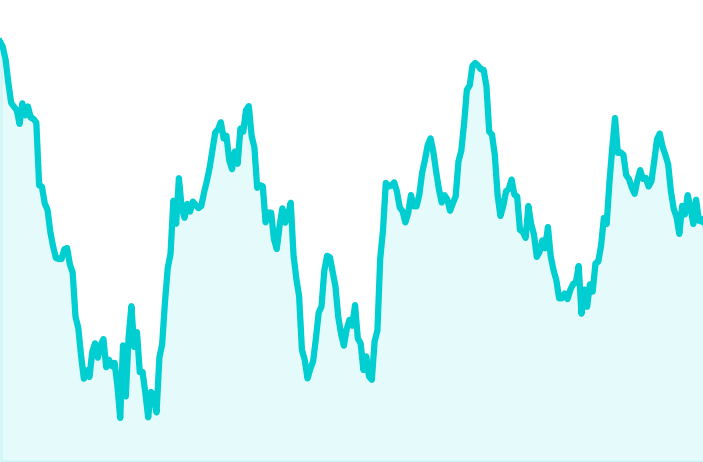
\includegraphics[
				width=2cm,
				height=2cm
				]{assets/images/waveform.png}};

			\node[below=0.15cm of input, font=\small] {Input};

			% STFT
			\node[imgbox] (stft) at (3.5,0)
			{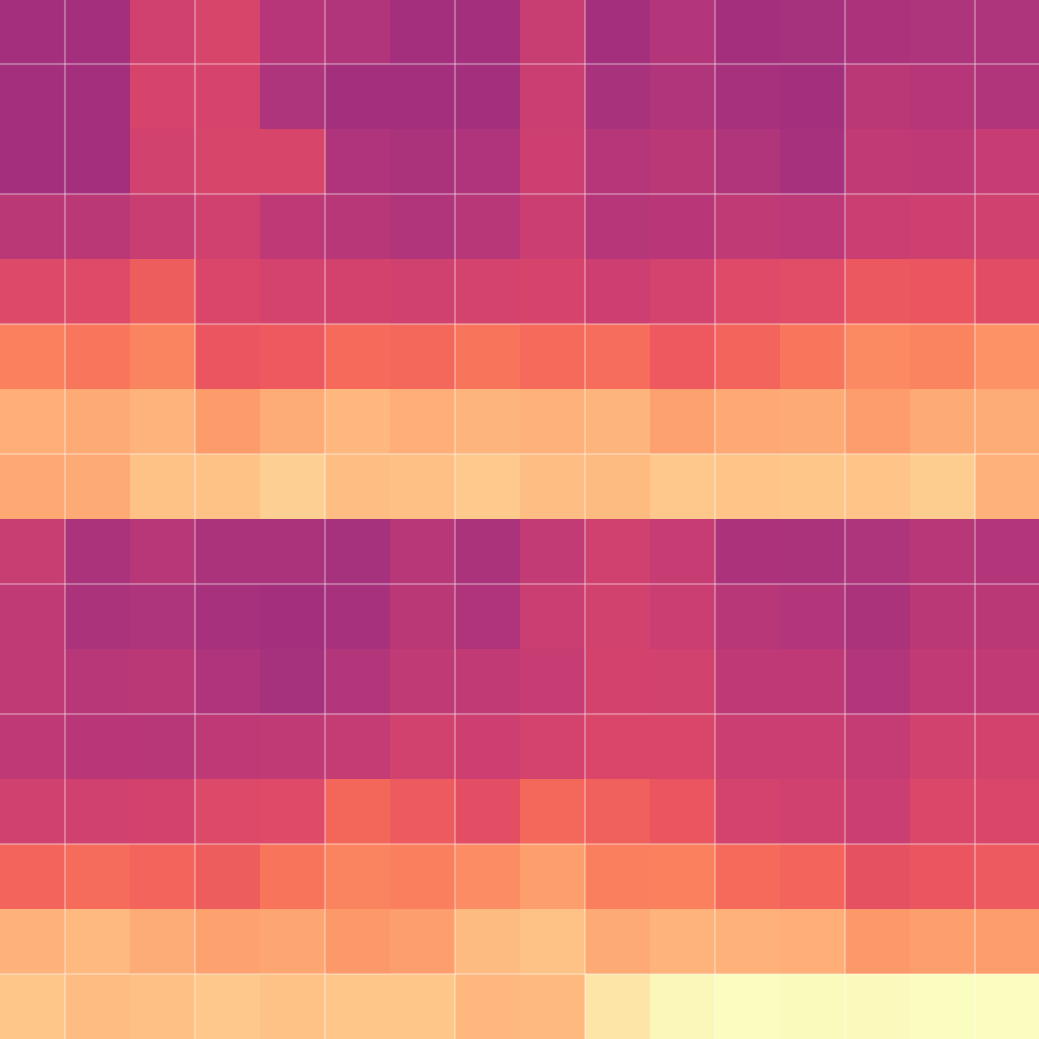
\includegraphics[
				width=2cm,
				height=2cm
				]{assets/images/spectrogram3.png}};

			\node[below=0.15cm of stft, font=\small] {STFT};

			\draw[solid arr]
			(input.east) -- (stft.west);

			% Router e Memoria
			\node[box] (router) at (7.0,1.6) {Router};
			\node[box] (memory) at (7.0,-1.6) {Memoria};

			% Split principale dopo STFT (Est)
			\coordinate (stft_split) at (5.2,0);

			\draw[thick]
			(stft.east) -- (stft_split);

			% STFT -> Router
			\draw[solid arr]
			(stft_split)
			-- (5.2,1.6)
			-- (router.west);

			% STFT -> Memoria
			\draw[solid arr]
			(stft_split)
			-- (5.2,-1.6)
			-- (memory.west);

			% Memoria -> Router (concat)
			\draw[dashed arr]
			(memory.north)
			-- (router.south)
			node[midway,right,font=\footnotesize] {concat};

			% Modelli
			\node[box] (mod1) at (12.5,1.6) {Modello 1};
			\node[font=\Huge] (dots) at (12.5,0) {$\vdots$};
			\node[box] (modN) at (12.5,-1.6) {Modello $N$};

			% Ingressi Modello 1: STFT (alto), Router (centro), Memoria (basso)
			\coordinate (m1_stft)   at (11.3,1.76);
			\coordinate (m1_router) at (11.3,1.60);
			\coordinate (m1_mem)    at (11.3,1.44);

			% Ingressi Modello N: STFT (alto), Memoria (centro), Router (basso)
			\coordinate (mN_stft)   at (11.3,-1.44);
			\coordinate (mN_mem)    at (11.3,-1.60);
			\coordinate (mN_router) at (11.3,-1.76);

			% Router -> modelli (Trunk a x=9.5)
			\coordinate (router_split) at (9.5,1.6);

			% Verso Modello 1 (dritto al centro: y=1.60)
			\draw[double line, ->]
			(router.east) -- (router_split) -- (m1_router);

			% Verso Modello N (scende alla porta inferiore: y=-1.76)
			\draw[double line, ->]
			(router.east) -- (router_split) |- (mN_router);

			% STFT -> Modelli e snstruction Error (percorso inferiore)
			\coordinate (model_recon_split) at (10.0,-4.2);

			% Da stft_split scende a -4.2 e va a destra fino allo split
			\draw[thick]
			(stft_split) -- (5.2,-4.2) -- (model_recon_split);

			% STFT -> Modello 1 (Porta superiore: y=1.76)
			\draw[solid arr]
			(model_recon_split)
			-- (10.0,1.76)
			-- (m1_stft);

			% STFT -> Modello N (Porta superiore: y=-1.44)
			\draw[solid arr]
			(model_recon_split)
			-- (10.0,-1.44)
			-- (mN_stft);

			% Memoria -> modelli (Trunk a x=10.5)
			% Linea perfettamente orizzontale da memory.east (y=-1.60) fino a x=10.5
			\coordinate (memory_split) at (10.5,-1.6);

			\draw[dashed,thick]
			(memory.east) -- (memory_split);

			% Da x=10.5 sale verso Modello 1 (Porta inferiore: y=1.44)
			\draw[dashed arr]
			(memory_split)
			-- (10.5,1.44)
			-- (m1_mem);

			% Da x=10.5 va dritto verso Modello N (Porta centrale: y=-1.60)
			\draw[dashed arr]
			(memory_split) -- (mN_mem);

			% Output
			\node[imgbox] (output) at (16.0,1.6)
			{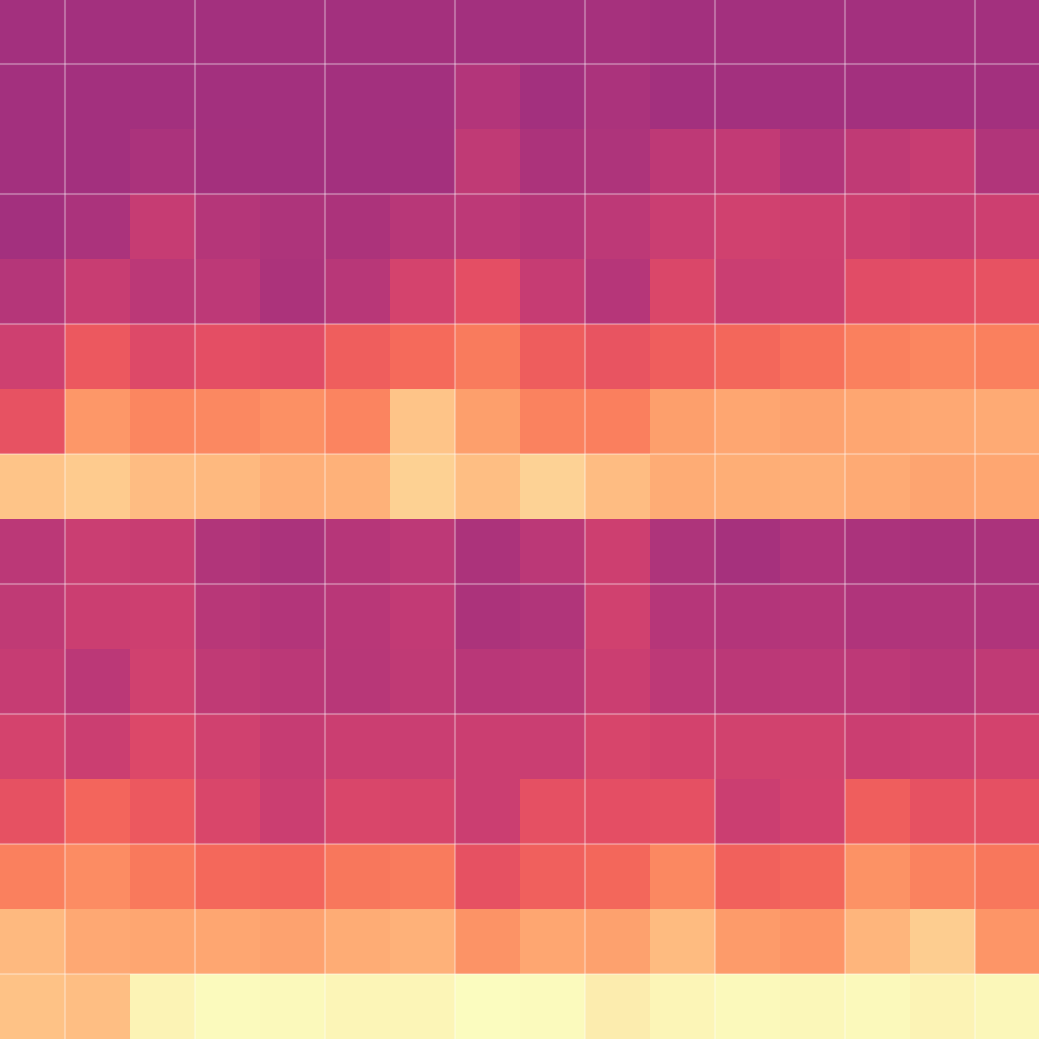
\includegraphics[
				width=2cm,
				height=2cm
				]{assets/images/spectrogram4.png}};

			\node[below=0.15cm of output, font=\small]
			{Output Selezionato};

			\draw[solid arr]
			(mod1.east) -- (output.west);

			% Reconstruction Error
			\node[
			box,
			fill=gray!10
			] (recon) at (16.0,-4.2)
			{Errore di \\ ricostruzione};

			% STFT -> Reconstruction Error (collegamento diretto orizzontale)
			\draw[solid arr]
			(model_recon_split) -- (recon.west);

			% Output -> Reconstruction Error
			\draw[solid arr]
			(output.south)
			-- (output.south |- recon.north)
			-- (recon.north);

			% Legenda
			\node[
			draw,
			thick,
			rounded corners=2pt,
			fill=white,
			align=left,
			inner sep=6pt,
			font=\footnotesize
			] at (7.5,-5.85)
			{%
				\textbf{Legenda}\\[3pt]
				\tikz[baseline=-0.5ex]
				\draw[thick,->] (0,0) -- (0.8,0);
				\quad Flusso principale\\[4pt]
				\tikz[baseline=-0.5ex]
				\draw[double,double distance=2pt,thick,->]
				(0,0) -- (0.8,0);
				\quad Selezione modello (argmax)\\[4pt]
				\tikz[baseline=-0.5ex]
				\draw[dashed,thick,->] (0,0) -- (0.8,0);
				\quad Memoria (opzionale)
			};

		\end{tikzpicture}%
	}
	\caption{Architettura del \textit{ensemble}.}
	\label{fig:architecture}
\end{figure}
